\documentclass[UTF8]{ctexart}
\usepackage{geometry, CJKutf8}
\geometry{margin=1.5cm, vmargin={0pt,1cm}}
\setlength{\topmargin}{-1cm}
\setlength{\paperheight}{29.7cm}
\setlength{\textheight}{25.3cm}

% useful packages.
\usepackage{amsfonts}
\usepackage{amsmath}
\usepackage{amssymb}
\usepackage{amsthm}
\usepackage{enumerate}
\usepackage{graphicx}
\usepackage{multicol}
\usepackage{fancyhdr}
\usepackage{layout}
\usepackage{listings}
\usepackage{float, caption}

\lstset{
    basicstyle=\ttfamily, basewidth=0.5em
}

% some common command
\newcommand{\dif}{\mathrm{d}}
\newcommand{\avg}[1]{\left\langle #1 \right\rangle}
\newcommand{\difFrac}[2]{\frac{\dif #1}{\dif #2}}
\newcommand{\pdfFrac}[2]{\frac{\partial #1}{\partial #2}}
\newcommand{\OFL}{\mathrm{OFL}}
\newcommand{\UFL}{\mathrm{UFL}}
\newcommand{\fl}{\mathrm{fl}}
\newcommand{\op}{\odot}
\newcommand{\Eabs}{E_{\mathrm{abs}}}
\newcommand{\Erel}{E_{\mathrm{rel}}}

\begin{document}

\pagestyle{fancy}
\fancyhead{}
\lhead{陈立冬, 3220105781}
\chead{数据结构与算法项目作业:四则混合运算器}
\rhead{\today}

\section{测试程序的设计思路}

本代码借助栈来实现表达式的四则运算。一共设立两个栈:values和operators,分别存放数字和操作符,且将操作符划分等级,依次读取输入的字符,并识别是数字还是操作符,分别放入相应的栈中。若入栈的操作符优先级比栈顶的低,则弹出栈顶操作符和两个操作数进行计算,并将结果重新放入数字栈中。

实现的功能:
\begin{itemize}
    \item 支持多重括号和四则运算。
    \item 支持有限位小数运算。
    \item 识别非法的表达式:括号不匹配、运算符连续使用、表达式以运算符开头或结尾以及除数是 0 等。
    \item 允许进行负数运算。
    \item 考虑了科学计数法。
\end{itemize}

定义类ExpressionEvaluator,暴露公共接口:static double evaluate(const std::string& expression);用于计算表达式计算结果

数据读入:输入的数据以字符串的方式储存,调用函数读取字符串并跳过空格,按字符读入数据并调用函数执行相应的操作。

小数处理:将小数点看作数字的一部分,在读入数字的过程中直接读入。

非法格式处理:定义变量expectOperator用于储存下一个期望读入的数据类型(如当前读入了数字,则expectOperator=true,及下一个期望读入的是操作符;如当前读入了操作符,则expectOperator=false,及下一个期望读入的是数字),如果期望读入数字而读到了操作符,则判定操作符非法。这样可以解决多个操作符和操作符位于开头的错误。
在读入栈顶元素前会先检测栈是否非空,若栈空会抛出错误,这样可以实现判断操作符多于操作数的错误(如2+2+,以及(2+2)

负数处理:作符非法时,如果操作符是负数,则该操作符为负号而非减号,将符号标志位sgn=-1,该标志位会乘以数字而得到负数的结果。

科学计数法处理:将e当作优先级最高的操作符进行计算即可。

\section{测试的结果}

自己写了个runTests()函数进行功能测试,测试结果如下:

\begin{figure}[h]
    \centering
    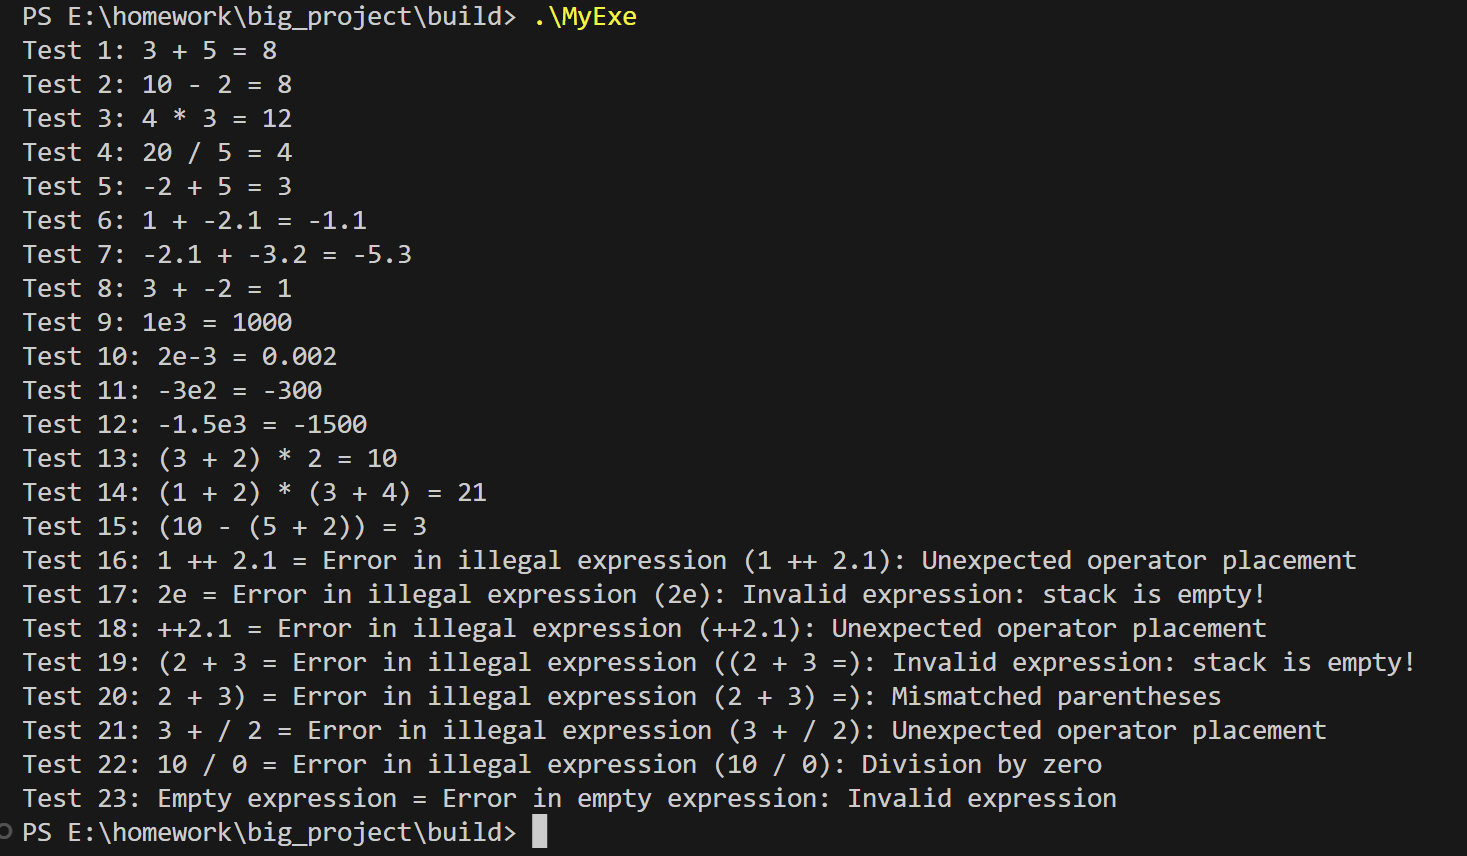
\includegraphics[width=0.5\linewidth]{image.png}
    \caption{测试结果}
    \label{fig:enter-label}
\end{figure}


可以看到代码对加减乘除四则运算,括号运算,小数、负数、科学计数都可以得出正确结果。且在多个运算符,开头结尾有运算符,括号缺省等错误格式有相应的报错。

\end{document}

%%% Local Variables: 
%%% mode: latex
%%% TeX-master: t
%%% End: 
